\subsection{Линейные формы (функционалы). Сопряженное (дуальное) пространство. Контрвариантный и ковариантный законы преобразования координат.}

\deff{def:} $V$ - линейное пространство над полем $K$, $f:V \rightarrow  K$ - линейная:
$$\forall \lambda \in K: \forall  v_1,v_2 \in V: f(v_1+ \lambda v_2) = f(v_1)+ \lambda f(v_2)$$
Такое $f$ называется \deff{линейной формой} или \deff{функционал}.

\textbf{Примеры:}

\begin{enumerate}
    \item $\overline{b} = const: \forall \overline{a}: \in V_3: f(\overline{a}) = (\overline{a},\overline{b})$ - очевидно линейная форма
    \item $A_{n\times n}: f(A) = tr (A)$ - очевидно линейная.
    \item $p \in P$, $\, t_0 \in k \text{ фикс.} \, f(p)= \frac{p^{(m)}t_0}{m!}$ - линейная форма.
    \item $f\in \mathbf{C}(\mathbf{R})$ - бесконечномерное линейное пр-во. $\delta(f)=f(0)$ --- дельта-функция Дирака.
\end{enumerate}

$f_1, f_2$ - линейные формы. Введем операции:
\begin{enumerate}
    \item \textbf{Сложение:} $(f_1+f_2)(v) = f_1(v) + f_2(v)$
    \item \textbf{Умножение на скаляр:}  $(\lambda f_1) (v) = \lambda f_1(v)$
\end{enumerate}
Очевидно существует ноль и противоположные. Откуда выполнены аксиомы 1-8, откуда линейное пространство. 

$V^* = \{f: V \rightarrow K \text{ - линейная форма}\}$ - называется \deff{сопряженное} пр-во к $V$ или \deff{дуальное}.

Возьмем $V$, зафиксируем  $e_1,\ldots,e_n$ - базис.

$\forall X \in V: X\in \sum\limits_{i=1}^nx_i e_i = x^ie_i$ - вспоминаем правило Энштейна из первого семестра. Тогда:
$$X \xleftrightarrow{e}\begin{pmatrix}
    x^1 \\
    x^2 \\
    \vdots \\
    x^n
\end{pmatrix} =x$$ 
$f(X) = f(x^ie_i) = x^if(e_i) = x^ia_i$, где $f(e_i) = a_i \in K$. $f(X) = a_1x^1+a_2x^2 + \ldots + a_n x^n$.

$f \leftrightarrow a= (a_1,\ldots, a_n)$ строка. %Цитата: то есть теперь  у нас функции описываются строками, расписать более подробно(это я себе)
$V^* = (K^n)^T$. 

Откуда $\dim V^*  = n$. 
Это взаимооднозначное соответствие, оно очевидно линейно, откуда это изоморфизм.

То есть теперь на самом деле функции описываются строками --- значениями на базисных векторах.



\textbf{Пример:} 

 Возьмем и посмотрим на скалярное произведение в
$V_3, \, \bar{b}= const$. $\forall X \in V_3, \, f(\bar{X})=(\bar{X}, \bar{b})$.

$f(\bar{i})=(\bar{i}, \bar{b}) = b_1$, $f(\bar{j})=(\bar{j}, \bar{b}) = b_2$, $f(\bar{k})=(\bar{k}, \bar{b}) = b_3$

$\bar{X}=a_1\bar{i}+a_2\bar{j}+a_3\bar{k}$

$f(\bar{X})=a_1b_1+a_2b_2+a_3b_3, $ у нас строка $f \leftrightarrow (b_1,b_2,b_3)$

\deff{def:} $V$, $e = (e_1,\ldots, e_n)$ базис.

$\forall x \in V: w^i(x) = x^i$ --- $i$-ая координата вектора $x$ относительно базиса e.  

$w^i$ называется \deff{координатной функцией}.

Не трудно заметить, что $w^i$ - линейная форма $\in V^{*}$.

\thmm{Теорема 1: (о базисе $V^*$)}

Доказать $w^1,\ldots,w^n$ - базис $V^*$.

\textbf{Доказательство:}

Докажем порождаемость: 

$\forall f \in V^*: \forall x \in V: f(x) = x^i a_i = w^i(x)a_i$, где $a_i \in K$ --- порождаемое

Докажем линейную независимость, показав единственность разложения нуля:

$\zero = \alpha_i w^i $, где $\alpha_i \in K$. Посмотрим на $\forall x \in V: \, \alpha_iw^i(x)=\zero$.

Пусть $x = e_j$ для $j = 1,\ldots, n$. Как мы знаем, для $i\neq j: w^i(e_j) = 0$. Тогда $\alpha_iw^i(e_j)=\alpha_j =0$,
$\forall j \Rightarrow $лин. независим.

\hfill Q.E.D.

\textbf{Следствие:} $w^i$ координатные формы относительно базиса $e$
$\Rightarrow \forall f \in V^*: f = a_iw^i$, т.е $a=(a_1,\ldots,a_n)$  координаты $f$ в базисе $w = (w^1,\ldots, w^n)$ пространства $V^*$


\deff{def:} $w^1,\ldots, w^n$ называется \deff{сопряженным} (дуальным) к базису $e$ пространства $V$.

Очевидно $w^j(e_j) = \sigma^i_j$.

\thmm{Теорема 2:}

$\forall$ базиса $w'^1,\ldots, w'^n$ пространства $V^*$.

$\exists!$ базис $e'_1, \ldots, e'_n$ пространства $V$ такой, что $w'$ базис, сопряженный к $e'$. То есть $w'^{i} $ координаты формы относительно $e'$.

\textbf{Доказательство:}


Пусть $e_1,\dots ,e_n \text{ базис } V$. Тогда, как мы говорили ранее:
$ w^1,\dots,w^n $ координатные функции относительно $e$, базис $V^*$ сопряженный к $e$.

Возьмем $w'$. Так как он базис и $w$ базис, то: $$ w' =wT_{w \rightarrow w'}$$
$(T_{w \to w'})^T=S=(S^i_j)_{n\times n}$. Заметим, что $S$ не вырожденная, т.к. $T$ матрица перехода. Строки матрицы $S$ - это координаты элементов нового базиса $w'$ в старом базисе($w$).
$$(w'^1,\ldots,w'^n)=(w^1,\ldots,w^n)T_{w \to w'}$$
Давайте все транспонируем:
$$\begin{pmatrix}
    w'^1 \\
    \vdots \\
    {w'}^n
\end{pmatrix} = (T_{w \to w'})^T \begin{pmatrix}
    w^1 \\
    \vdots \\
    {w}^n
\end{pmatrix}= S \begin{pmatrix}
    w^1 \\
    \vdots \\
    {w}^n
\end{pmatrix}$$
Пусть $S^{-1}=T=(t^i_j)_{n \times n}$ - невырожденная, то если думать о ней как о $T_{e \to e'}$, получим, что $ e' = eT$ базис в пр-ве $V$.

Осталось показать, что $w'$ будет сопряженным к $e'$, т.е. показать ${w'}^{ i}(x)={x'}^i, \, x = {x'}^i {e'}_i$, для всех $ x \in V$. Тк $w'^i$ - линейная форма, то:
$${w'}^i({x'}^i{e'}_j)= {x'}^j {w'}^i(e'_j)$$
Теперь, давайте заметим, что ${w'}^i=S^i_kw^k$, $e'_j = t^m_je_m$. Откуда 
$$ {w'}^i(e'_j)=  S^i_kw^k(t^m_je_m)  = S_k^jt_{j}^m w^k(e_m) = S^i_mt^m_j=(ST)^i_j = $$
\hfill Q.E.D.

\textbf{Следствие.} $e,e'$ базисы $V$, $w,w'$ сооответственные сопряженные базисы к $e,e'$ в $V^*$.

$T = T_{e\rightarrow e'}, S = T^{-1}$

$ \Rightarrow \forall x \in V: \forall f \in V^*:x' = Sx, a' = aT$, где $a$ - разложение $f$ в базисе.

\textbf{Доказательство:}

$T=T_{e\rightarrow e'}$ и мы уже знаем, что $x' = T_{e'\rightarrow e}x = Sx$ 

$(T_{w\rightarrow w'})^T = S$. Как мы знаем из матрицы перехода:
$$a^T = T_{w\rightarrow w'}(a')^T$$ 
Откуда:
$$a = a'(T_{w\rightarrow w'})^T = a'S$$
А уже отсюда получаем, что $a' = aS^{-1} = aT$.

\hfill Q.E.D.

\textbf{Замечание от Славы.} Очень удобно менять базис, когда у нас один из базисов канонический. А также, зная матрицу перехода $T_{w\rightarrow w'}$ мы уже знаем матрицу перехода из $T_{e\rightarrow e'} =((T_{w\rightarrow w'})^T)^{-1} $


Преобразование координат, согласованных по тому же закону, что и базис:
$a' =a T$

Преобразование координат, согласованных по противоположному закону:
$x' = Sx$

\deff{def:} Преобразование координат векторов пространства $V$ происходит по закону, противоположному преобразованию базисов --- называется \deff{контрвариантным}, а координаты векторов пространства $V$ называется \deff{контрвариантыми}(индексы координат пишутся сверху)

\deff{def:} Преобразование координат векторов пространства $V$ происходит по тому же закону, что преобразованию базисов в пространстве $V$(т.е. согласованно) называется \deff{ковариантным} преобразованиям.
Координаты векторов пространства $V^* $ называется \deff{ковариантным}(индексы пишутся внизу)

Позамечаем интересные факты:

$\forall f \in V^* \leftrightarrow (a_1,\ldots, a_n), a_j = f(e_j)$ - каждой функции, как и говорилось ранее, на заданном базисе, я могу сопоставить $a$. Поэтому возьму $n$ функций и векторов, и захочу посчитать значение каждой функции в каждой точке : 

$\forall f^1, \ldots f^n \in V^*: f^j \xleftrightarrow{w} a^j = (a_1^j,\ldots , a_n^j)$

$\forall x_1, \ldots, x_n \in V: x_i \xleftrightarrow{e}x_i = \begin{pmatrix}
    x^1_i \\
    \vdots \\ 
    x^n_i
\end{pmatrix}$

Хочу посчитать вот такую вот страшную матрицу (значение каждой функции в каждой точке):

$(f^j(x_i))_{n\times n} = \begin{pmatrix}
    f^1(x_1) & f^1(x_2) & \dots & f^1(x_n)\\
    f^2(x_1) & f^2(x_2) & \dots & f^2(x_n)\\
    \vdots & \ddots & \ddots & \vdots \\
    f^n(x_1) & f^n(x_2) & \dots & f^n(x_n)\\
\end{pmatrix} = f^j(x_i)= a^j x_i  = $


$=\begin{pmatrix}
    a_1^1 & \ldots & \ldots& a^1_n\\ 
     a_1^2 & \ddots & \ddots& a^2_n\\ 
      \vdots & \ddots & \ddots& \vdots\\ 
      a_1^n & \ldots & \ldots& a^n_n\\ 
\end{pmatrix} \cdot\begin{pmatrix}
    x_1^1 & \ldots & \ldots& x^1_n\\ 
     x_1^2 & \ddots & \ddots& x^2_n\\ 
      \vdots & \ddots & \ddots& \vdots\\ 
      x_1^n & \ldots & \ldots& x^n_n\\ 
\end{pmatrix} = \begin{pmatrix}
    f^1\\
    f^2\\
    \vdots\\
    f^n
\end{pmatrix} \cdot \begin{pmatrix}
    x_1 & x_2 & \ldots & x_n
\end{pmatrix}$ - лаконичная запись!



Интересный факт, который идет из такого произведения:
$$\begin{pmatrix}
    w^1 \\
    w^2 \\
    \vdots \\
    w^n \\
\end{pmatrix} \cdot (e_1e_2 \dots e_n) = E $$

\deff{def:} $V^{**} = (V^*)^*$ \deff{дважды сопряженное} пространство.

$\forall f \in V^*$. Пусть $x \in V$:

$"x"(f) = f(x)$. $"x": V^* \rightarrow K$.

$\forall \lambda \in K: \forall f^1,f^2 \in V^*$

$"x"(\lambda f^1+f^2) = (\lambda f^1 + f^2)(x) = \lambda f^1(x) + f^2(x) = \lambda_1 "x"(f^1) + "x"(f^2)$

$\Rightarrow "x"$ линейное отображение $\Rightarrow"x" \in (V^*)^*$

Дальше у $"x"$ будут упускаться "" :))

\thmm{Теорема 3 (О естественном изоморфизме)}

Естественный - не зависит от введения базиса.

$V \cong V^{**}$

\textbf{Доказательство:}

$\forall x \in V \rightarrow "x"\in V^{**}$. Назовем это отображение $\varphi$.

Покажем, что наше взаимооднозначное сопоставление линейно.

$x_1 + \lambda x_2 \in V: x_1 \rightarrow "x_1"$, $x_2 \rightarrow "x_2"$


$\forall f\in V^*: "x_1+\lambda x_2"(f) = f(x_1+\lambda x_2) = f(x_1) + \lambda f(x_2) = "x_1"(f) + \lambda"x_2"(f) $. Откуда $\varphi$ линейно.

\begin{center}
    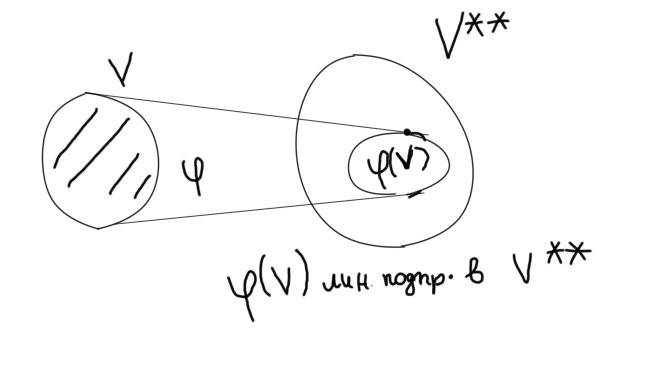
\includegraphics[width =15cm]{assets/8_1-varphi-linear.png}
\end{center}

Покажем, что $\varphi$, это изоморфизм.

Пусть $e_1,\ldots, e_n$ базис $V$. Им соответствуют $ "e_1"$$,\ldots, "e_n"$. Покажем, что это базис в $V^{**}$:

Мы знаем, что $\dim (V^*)^* = \dim V^* = \dim V = n$. Откуда достаточно показать, что $"e_1"$ $,\ldots, "e_n"$ - линейно независимы. Для этого покажем единственность разложения нуля.

$0= \sum\limits_{i=1}^n \alpha_i "e_i"(w_i)=\sum\limits_{i=1}^n\alpha_i w^j(e_j) = \alpha_j \Rightarrow$ линейно независимы, откуда базис.

Откуда отображение $\varphi$ это изоморфизм.

\hfill Q.E.D.

Как мы только что поняли: $x \in V \leftrightarrow "x" \in V^{**}$ - изомофризм. $f\in V^{*}, x \in V$.

$x(f)= f(x) = x^i a_i = w^i(x) a_i = x(w^i)a_i =x^ia_i=x^i f(e_i)=x^ie_i(f)$

$e \text{ и }w$ взаимно сопряж.

$x=x^ie_i, w^i(x)=x^i,$ где $x \in V$

$e_j(f)=f(e_j)=a_j(f \in V^*)$, $e_j \in V^{**}$ - коорд. формы относительно базиса $w^i$.

Я категорически не помню для чего Кучерук это написала, напомните мне пж.





\textbf{Пример:}

$\mathcal{A}$ - о.п.с, $A$ - диагонализируема.

$V = \bigoplus\limits_{\lambda}V_{\lambda} = \span (v_1,\ldots,v_n)$

$w^1,\ldots,w^n$ сопряж. базис к $v$  % дописать

$\Rightarrow \forall x \in V: w^j(x) =x^i: x^iv_j = x$ 

\newpage
\subsection{Два определения тензора. Линейное пространство тензоров. Многомерная матрица тензоров.}

\deff{def:} Есть $V,V^*$ и $p,q \in N$.

\deff{Тензором} типа $(p,q)$ ($p$-раз коварентная, $q$-раз контрвариантным) называется полинейная функция $f: V^p\times (V^*)^q \rightarrow K$. $p,q$ называются \deff{валентностями} тензора, $r = (p+q)$ ранг тензора.

Если $r = 0, f = const$. Если тензор $(p,0) $ - \deff{ковариантный} тензор валентности $p$. Если тензор $(0,q)$ - \deff{контрвариантный} тензор валентности $q$. $p\neq 0 $ и $q\neq 0$ - тензор смешанного типа.

$\xi_j \in v, \eta^i \in V^*$

$f(\xi_1,\ldots,\xi_p,\eta^1,\ldots, \eta^q)$ - линейно по каждому аргументу

$e = (e_1,\ldots, e_n)$ - базис $V$

$w = (w^1,\ldots, w^n)$ - базис $V^*$

$\xi_j = \xi_j^{j_k}e_{j_k}$

$\eta^i = \eta_{i_m}^iw^{i_m}$

$f(\xi_1,\ldots,\xi_p,\eta^1,\ldots, \eta^q) = \xi_1^{j_1}\ldots\xi_p^{j_p}\eta_{i_1}^1 \ldots \eta^q_{i_q} \cdot f(\xi_{j_1},\ldots, \xi_{j_p},w^{i_1},\ldots, w^{i_n})$

%тут что-то пропщено я потерялся в мире

\deff{def:} $M$ - многомерная матрица $r = (p+q)$ мерная  размерности $n$. %Что блять?
